\insertmeeting 
	{More CAD} 
	{09-22-22}
	{Hagerty High School}
	{Jensen, Jorge, Karissa, Laura, Nathan, Robert, Samantha, Tyler}
	{Images/RobotPics/robot.jpg}
	{2:30 - 4:00}
	
\hhscommittee{Hardware}
\noindent\hfil\rule{\textwidth}{.4pt}\hfil
\subsubsection*{Goals}
\begin{itemize}
    \item Assemble the field

\end{itemize} 

\noindent\hfil\rule{\textwidth}{.4pt}\hfil

\subsubsection*{Accomplishments}
We've been waiting a while for our field parts to arrive, and today is finally the day that they have. Today was only spent assembling the field, using the official FTC instructions as our guide. An interesting limitation we came across was that we share our field with our VEX teams, who's game, Spin Up, divides sides of their field into diagonals. As such, the junctions we assembled could only go as far as the ones that laid on that diagonal. This meant we would only have 15/25 junctions in place. While this wasn't much of an issue for assembly, since VEX hadn't put the tape line usually in place on Spin Up fields, so we didn't need to remove anything. However, issues will arise when we start doing programming and driver practice, as we can't practice with the whole field. We're happy to finally have our field in place, but going forward, we need to be weary of potential oversights caused by this limitation, such as our limited ability to practice circuits, and programming autonomous for certain starting positions.



% \begin{figure}[htp]
% \centering
% 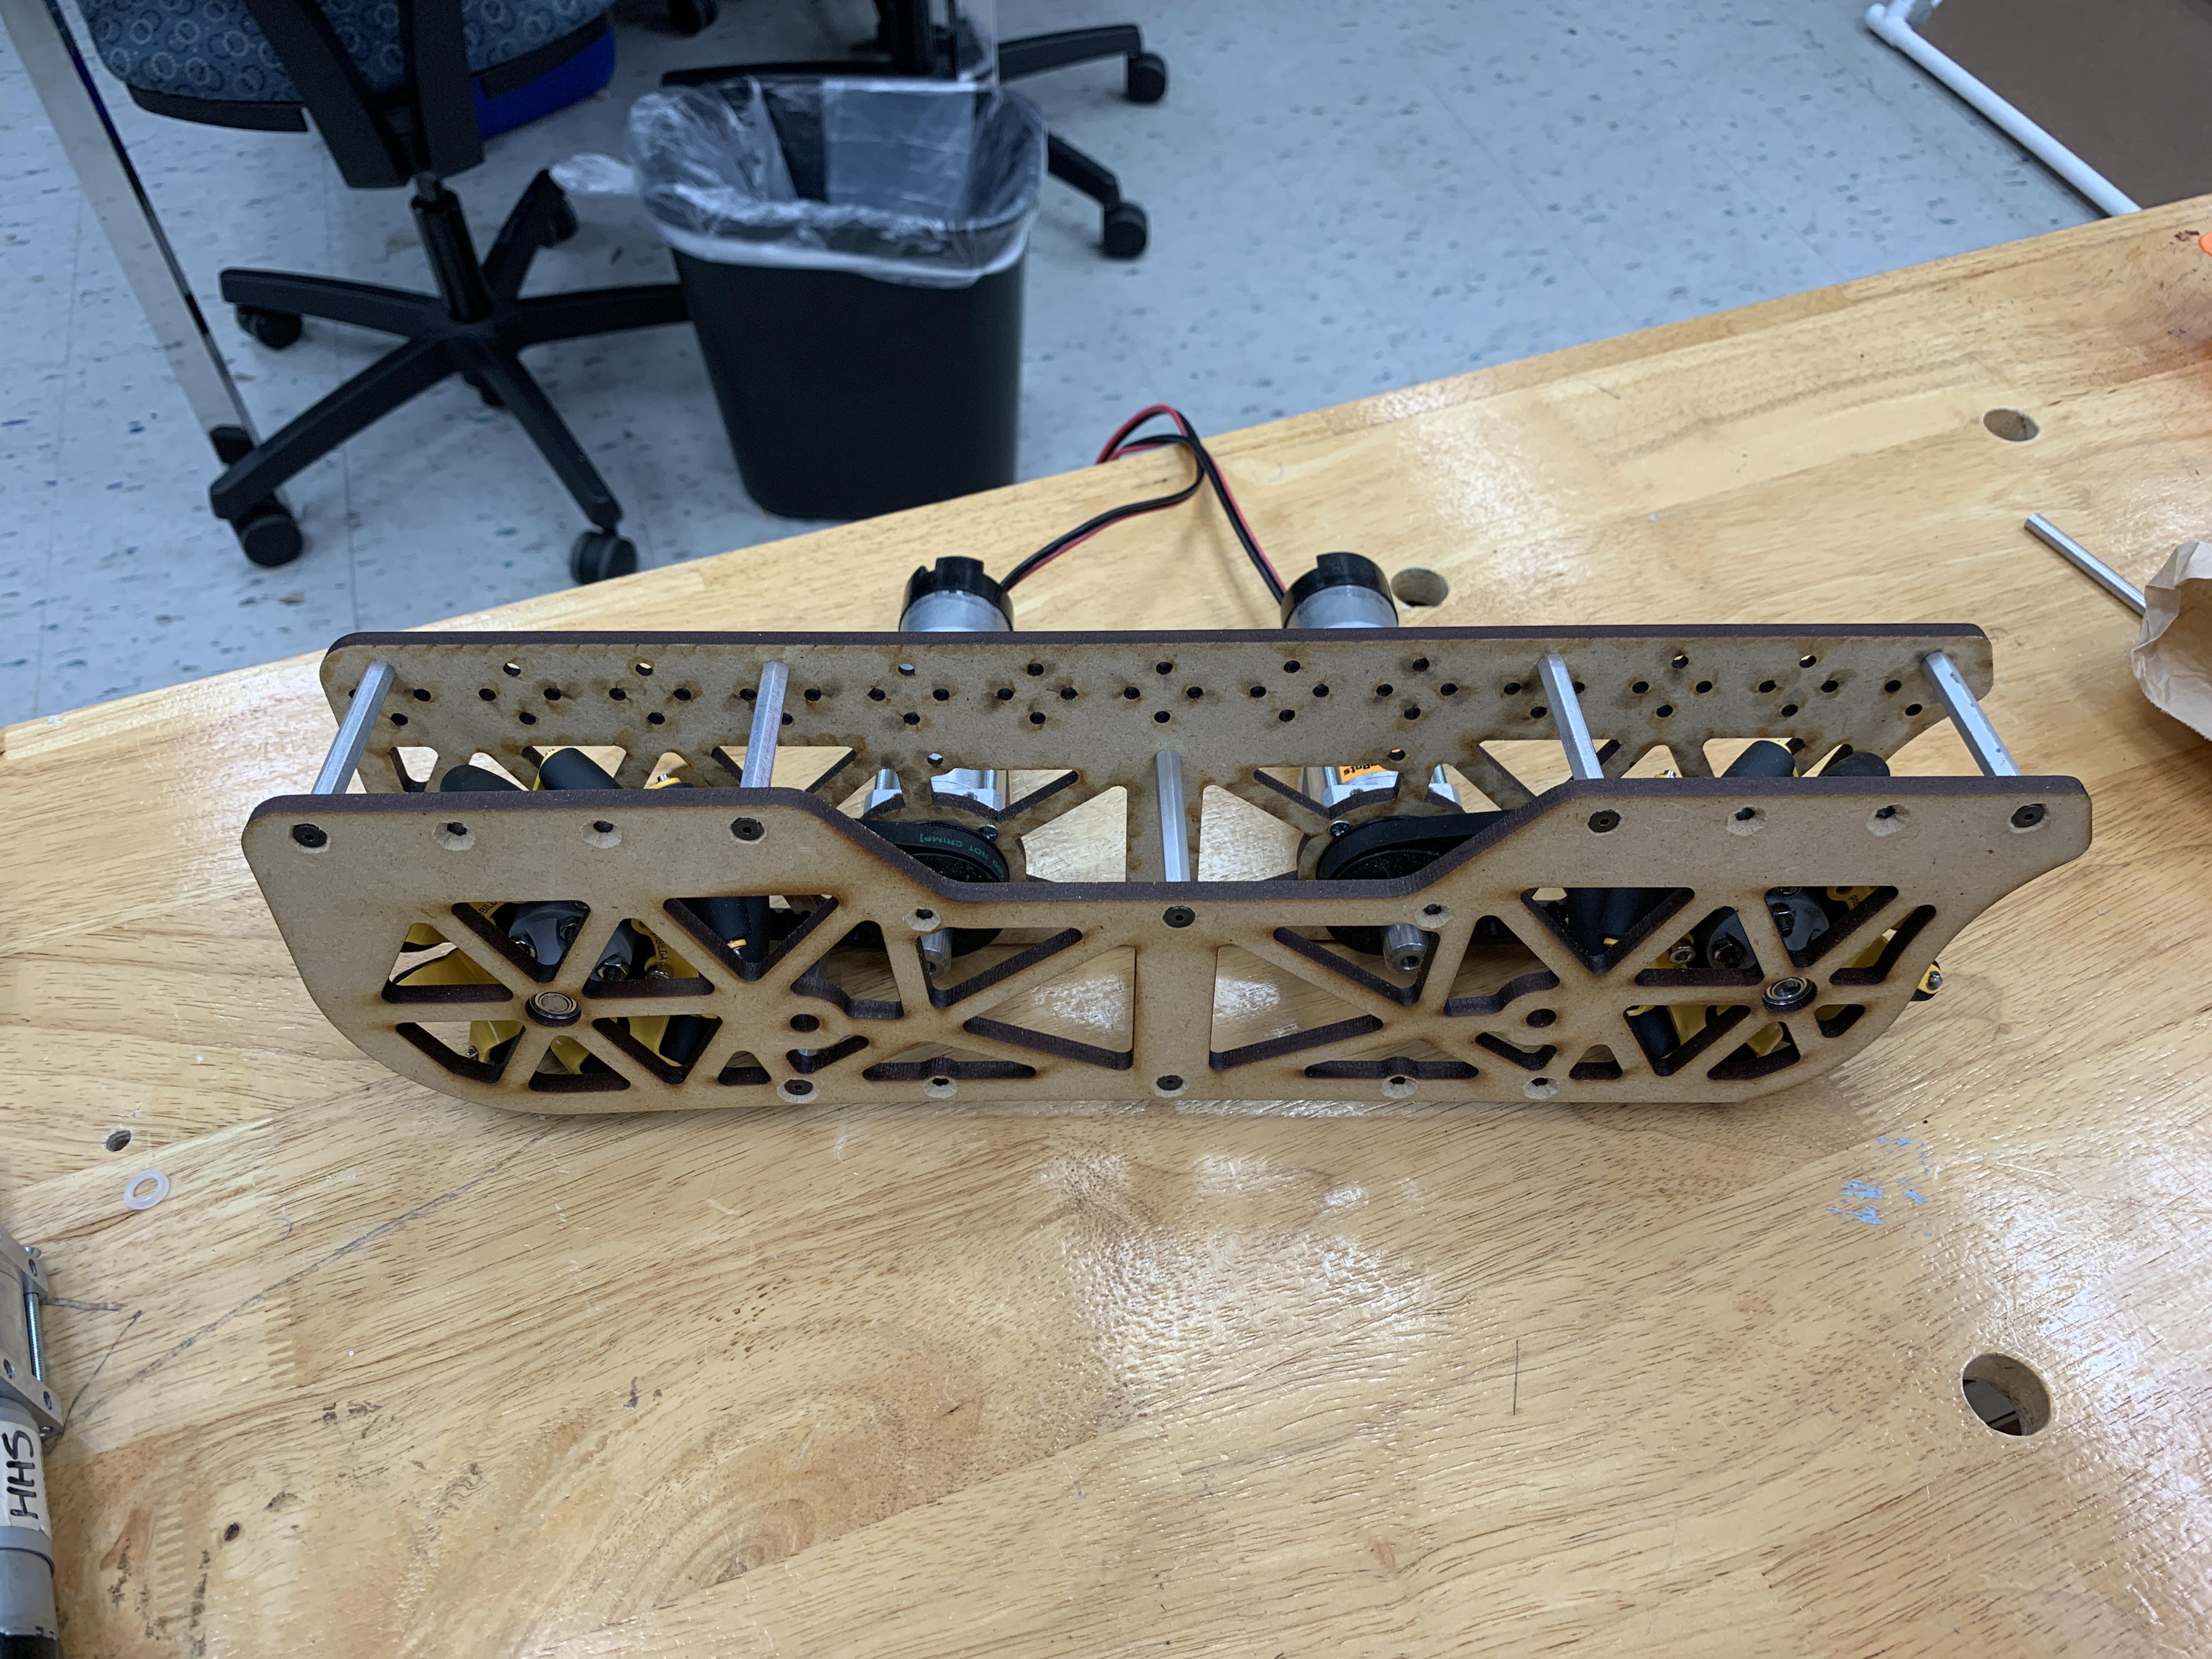
\includegraphics[width=0.9\textwidth, angle=0]{Meetings/July/07-21-21/drivetrain_7-20-21-NathanForrer.jpg}
% \caption{First half of the drivetrain.}
% \label{fig:072121_1}
% \end{figure}

\whatsnext{
\begin{itemize}
    \item CAD four bar intake
    
\end{itemize} 
}
